%% The following is a directive for TeXShop to indicate the main file
%%!TEX root = diss.tex

\chapter{Sediment transport and landscape evolution}
\label{ch:Introduction}

Landscapes evolve when water, wind, and ice, driven by gravity, grade the uplifted relics of forces from below Earth's surface.
Channels initiate along faults and depressions wherever climatic conditions are suitable, incising networks in the landscape and transferring sediments from uplands to lowlands as they grind them to sand through a machine of denundation.
Earth's biota colonize these networks which form conduits for migration, transmitting water and organic material while biota convert sediments to soils, staging the joint evolution of life and landscapes which has persisted over geological time.
Human impacts on these old patterns have become severe, in what has been characterized as an environmental and social crisis.
Geologic records display unprecedented recent shifts in ancient climatic, denundational, and biotic patterns, requiring effective aquatic habitat restoration, contaminant management, and river engineering strategies more than ever before.

In this context river geomorphology as a scientific practice is shifting toward more quantitative methods to enable concrete predictions about the natural world.
Sediment transport in river channels is especially amenable to this quantitative approach since it is basically the result of fluid and granular processes.
Modelling sediment transport is extremely challenging because fluid and granular physics are notoriously difficult subfields of classical physics.
Sediment moves in different modes depending on the relative importance of the fluid forces against the weight of grains.
When particles are coarse as in gravel-bed rivers, the fluid forces are relatively weak and particles move as ``bedload" by bouncing, rolling, and sliding along the bed surface. In these conditions, fluid turbulence and the irregular bed surface become important controls over sediment dynamics.

Bedload transport exerts considerable influence over stream morphology and stability \citep{Church2006,Hassan2008,Recking2016}, in part because the coarsest grains in a river provide a partially-immobile skeleton upon which sedimentary deposits can develop \citep{Zimmerman2007,Comiti2012, McKenzie2018, Eaton2020}.
As a result, a longstanding problem in river science is to determine the bedload flux, or downtream rate of movement of bedload sediment grains \citep{duBoys1879, }.
Unfortunately, existing approaches to compute the bedload flux are inadequate as predictions regularly deviate by orders of magnitude from measured values \citep{Gomez1989, Barry2004, Bathurst2007a, Recking2012, Dhont2018}, and this is despite well over a century of concerted effort \citep{Gomez1991}.
This state of affairs indicates that new research approaches are needed to accelerate research progress \citep{Ancey2020a,Ancey2020}.

Predicting bedload fluxes is challenging because transport is not always well correlated to average characteristics of the flow and bed material. 
Local fluxes can range through orders of magnitude as details of turbulent fluctuations and bed organization vary, while average characterizations of flow and sediment remain constant \citep{Sumer2003, Charru2004, Hassan2008, Venditti2017}.
The same turbulence and sediment organization details which correlate with the bedload flux also interact with it. 
Turbulent impulses drive sediment motion \citep{Valyrakis2010, Celik2014, Amir2014, Shih2017}, moving sediment affects turbulent flow characteristics \citep{Singh2010, Santos2014, Liu2016}, and bedload fluxes modify the stability and arrangement of bed surface grains \citep{Kirchener1990, Charru2004, Strom2008}, which encourages further transport in a positive feedback \citep{Ancey2008,Heyman2016,Lee2018}.
The bedload flux is thus in a cyclical feedback with its controls in the details of turbulence and bed organization \citep{Jerolmack2005}. 

The approach taken in this thesis is to consider the bedload flux as an aggregate result of many individual transported grains.
This departs from the traditional strategy of correlating transport rates to the mean flow and sedimentary characteristics \citep{Gilbert1917,MeyerPeter1948}.
Since the trajectories of individual grains are governed by Newtonian mechanics, this perspective provides a wide foothold on the problem.
The Newtonian approach is nonetheless complicated because the forces driving and resisting sediment motion vary through space and time, in part due to the turbulent flow and the erratic interactions of moving particles with the bed.
To address this complication, I develop in this thesis a handful of new bedload transport models using methods adopted from statistical physics.
These efforts build on an an earlier literature to provide more realistic descriptions of the trajectories of individual grains and the bedload fluxes they generate.

The thesis begins with a review of the most relevant pieces of this earlier literature on which my research builds. The rest of this chapter summarizes earlier works, rephrasing them when necessary to indicate common themes and to show continuity with my own research which follows in the subsequent chapters. In particular, the common theme to watch for is that many earlier models rely implicitly on the idealized noises of nonequilibrium statistical physics, Gaussian white noise, white Poisson noise, white dichotomous noise, and so on \citep{Cox1965,VanKampen1992,Gardiner1983,Kubo,Risken1984}. 
The review in this chapter focuses on two main themes: first, models of the movements of individual particles, and second, models of the over-all bedload flux which results from these individual movements. An outline of my own research which follows comes at the end of these two sections.

\section{Theories of individual particle movement}

A basic (but not simple) problem in sediment transport modelling is to predict the downstream movement of an individual particle.
At first glance, this seems an elementary problem in general physics, but challenges appear.
Particles moving as bedload are driven downstream by a turbulent fluid flow \citep{}, but the exact relationships between the fluid flow and the applied forces are not known \citep{Furbish1997}.
Downstream movement is resisted by frictional collisions between moving particles and the bed.
Since the bed is a granular surface, its surface geometry is very difficult to characterize \citep{Gordon1972}, and the outcome of collisions varies from one to the next \citep{Sekine1992}
Entrainment and deposition provide an additional layer of complexity.
Moving particles that encounter the bed with sufficiently low velocities can settle into pockets which protect them from the flow \citep{Miller1966} and they deposit \citep{Charru2004}.
These pockets are not permanent shelter, because rearrangement of the surrounding bed can re-expose particles to the flow, and sufficiently strong turbulent fluctuations can overcome shelter, even if it is not disturbed \citep{Valyrakis2012,Celik2014}, and particles entrain.
Ultimately, particles at rest on the bed surface can also become covered by other transported particles \citep{Yang1972}. These buried particles cannot move again until those burying them have been transported away \citep{Nakagawa1981}.

Individual trajectories of particles therefore involve a number of contributing processes, and we have limitations in our understanding of every one of these.
\citet{Nikora2001,Nikora2002} provided a conceptual model of individual particle motions which helps to organize earlier research by the subset of these processes which it attempts to incorporate, although this conceptual model been slightly revised in some recent studies \citep{Campagnol2013, Hassan2017, Pierce2020}.

Nikora et al divided the downstream trajectory of an individual particle into three timescales, or ``ranges", termed local, intermediate, and global.
The local range refers to the period of motion between subsequent interactions with the bed, when the particle accelerates downstream within the flow, the intermediate range reflects particle motions through sequences of collisions, and the global range refers to particle motion between subsequent entrainment and disentrainment events.
\citet{Hassan2017} added an additional range, referred to as ``geomorphic", to reflect the even longer period over which particles become buried. 
This set of timescales -- local, intermediate, global, and geomorphic -- provides a structure by which to organize wide modelling literature on bedload trajectories and to understand the approximations which have been made on the fundamental problem of predicting the downstream movements of individual grains.

\subsection{Motivation: tracers and basic understanding}
The original motivation to understand individual particle motions was probably to understand the efficiency of sediment transport measurements \citep{Ettema2004}, and this motivation still drives a great deal of research into individual particle motions today \citep{Hassan2017,Pretzlav2021}.
A common measurement technique to estimate sediment transport is to seed a stream with tracer stones and track their progress downstream \citep{Einstein1937, Takayama1966, Ashmore2020}.
In principle, tracers provide a proxy for the population of grains in a stream, so one can estimate tracer velocities of tracers, then multiply by an estimate of the number of grains available for motion in the stream to calculate the overall sediment flux \citep{Yano1969,Nakagawa1976,Hassan2017}.
In practice, challenges arise due to the distinct behavior of tracers over the local, intermediate, global, and geomorphic timescales. Apparently, tracer particle velocities depend on the observation time, in a phenomenon which has been called ``advective slowdown" \citep{Ferguson2002,Haschenberger2012}. This means it is not clear how measured tracer velocities can be mapped back to bulk sediment fluxes, exposing a need for further research into how exactly particle motion characteristics evolve through time.

This need to understand tracer movements is not however the sole point of research into individual particle motions. It is conceptually clear that bulk sediment fluxes ultimately result from the aggregated movements of individual grains, and the prediction of the sediment flux has long been acknowledged as a challenging problem with no clear solution, which impedes geomorphology and engineering understanding \citep{Ancey2020,Ancey2020a}. Better understanding of individual particle motions will support this research.

\subsection{Einstein 1937}
Einstein was probably the first to focus on the movements of individual particles through streams \citep{Einstein1937}, motivated (at least as far as his research supervisor Meyer-Peter was concerned) by the need to understand the efficiency of Helley-Smith samplers for the management of sedimentation \citep{Ettema2004}.
Watching painted tracers move through a flume, Einstein came to the conclusion that the movement characteristics of any one particle could not be predicted, so he turned to probabilistic methods to characterize their transport.
Einstein's key insight was to represent particle motions as an alternating sequence of movements and rests having random characteristics.
As his interest was on the global range of particle motion, and the duration of particle motions is usually short compared to rests, Einstein made the approximation that individual motions (between entrainment and deposition) are mathematically instantaneous.
With this configuration, the downstream movement of sediment becomes an alternate cycle of instantaneous steps of random length, separated by rests of random duration. 
Implicitly, this picture of sediment trajectories assumes that movement velocities are infinite.
Einstein's experiments indicated that both step lengths and resting times were well-described by exponential distributions, and the focus of his PhD was to find the probability density $P(x,t)$ that a particle had travelled a net distance $x$ after a time $t$ has elapsed. He formulated the problem mathematically with an infinite series of convolution integrals, in an elegant display of mathematical physics. 
The mathematics Einstein took on were a pioneering application of the continuous time random walk, which was not formalized until much later \citep{Montroll1965}.


For connection to later work in the thesis, and to provide additional perspective on Einstein's work which is not available in the literature, I will summarize Einstein's work slightly differently than he originally formulated it, using a method based on a stochastic dynamical equation.
In effect, if the position of a single sediment particle at a given time is $x(t)$, the assumptions of infinite movement velocity, random resting durations, and random movement distances between entrainment and depositon (step lengths) can be written
\be \dot{x}(t) = \mu(t), \label{eq:einlangevin}\ee
where $\dot{x} = dx/dt$, and $\mu(t)$ is a white shot noise \citep{VanDenBroeck1983}, which is essentially a sequence of pulses having random heights with mean height $\ell$ (the mean step length), and random locations in time with mean separation $1/k_E$ (the mean resting time, interpreted as the reciprocal of the entrainment rate $k_E$).
A particular realization of this pulsed noise can be written
\be \mu(t) = \sum_{i=1}^{N(t)}s_i \delta(t-t_i), \label{eq:einrando} \ee
where $N(t)$ is the number of particle entrainments in time $t$, distributed as a Poisson distribution $P(N) = e^{-k_E t} (k_E t)^N/N!$, the $t_i$ are distributed according to $P(t) = k_E\exp(-k_E t)$, and the $s_i$ are distributed according to $P(s) = \ell^{-1}\exp(-s \ell^{-1}).$
Figure \ref{fig:einsteinfig} panel (a) sketches this noise, and panel (b) sketches the resulting global range trajectory as a sequence of steps and rests.
Equation \ref{eq:einlangevin} is a kind of dynamical equation representing how the position of a sediment grain evolves through time \citep{Kubo1978}, similar in spirit to Newtonian mechanics \citep{Goldstein1956}, but with a particular random driving term (equation \ref{eq:einrando}) chosen to basically represent the phenomenon under consideration.

\begin{figure}[!htbp]
	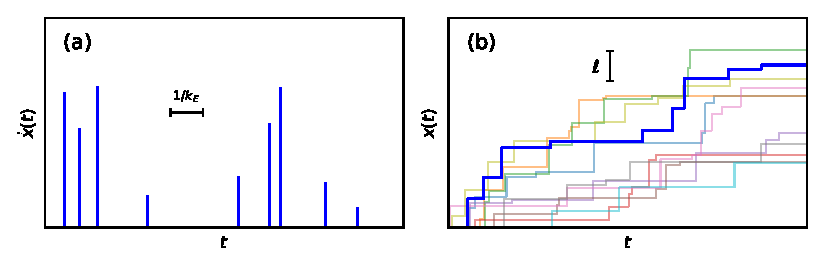
\includegraphics[width=\linewidth,keepaspectratio]{./figures/ch1/einsteinConcept.pdf}
	\caption{Panel (a) indicates the representation of Einstein's model as an idealized ``white shot noise", as indicated in eq. \ref{eq:einrando}, while panel (b) shows the ``stairstep" trajectories of sediment particles moving downstream through cycles of steps (which are instantaneous) and rests (which have mean duration $1/k_E$). }
	\label{fig:einsteinfig}
\end{figure}

The governing equation of the distribution $P(x,t)$ to find the particle at $x$ can be calculated as an ensemble average of $\delta(x-x(t))$ over all possible realizations of the noise \citep{Risken1984,Moss1989}. Different methods exist to compute such averages \citep{Hanggi1978, Hanggi1984, Balakrishnan1993, VanDenBroeck1983}, but whatever the approach, the governing equation for the distribution comes out as
\be  \big(\ell \px \pt + k_E \ell \px + pt \big)P(x,t) = 0. \label{eq:einmaster}\ee
This equation can be solved by standard methods (series solutions or transform calculus) \citep{Arfken1985,Prudnikov1986a} reproduce the original result of \citet{Einstein1937} for the probability distribution of position of a sediment particle:
\be P(x,t) = \delta(x) e^{-k_E t} + e^{-k_E t - x/\ell}\theta(x) \sqrt{\frac{k_E t}{\ell x}}\mathcal{I}_1\Big(2 \sqrt{\frac{k_E x t}{\ell}}\Big) \ee
Here, $\mathcal{I}$ is a modified Bessel function. 
The probability distribution eq. \ref{eq:eindist} fully characterizes the dynamics of an individual particle alternating through steps and rests. 

This distribution displays both advective and diffusive characteristics.
One can calculate all moments of the position by multiplying eq. \ref{eq:einmaster} by $x^n$ and integrating over space. This gives the mean position of the particle
\be \langle x \rangle (t) = k_E \ell t, \ee
so in Einstein's view, sediment grains move with effective velocity $V_\text{eff} = k_E \ell$, given by the entrainment rate times the mean step length.
The rate at which one particle spreads out from another due to differences in their motion characteristics can be represented by the variance of position, $\sigma_x^2  = \langle x^2 \rangle - \langle x \rangle^2$. This gives
\be \sigma_x^2(t) = 2 k_E \ell^2 t, \ee
so particles in Einstein's model spread apart as a normal diffusion process \citep{Sokolev2002}, with an effective diffusivity $D_\text{eff} = k_E \ell^2.$

\subsection{First extensions of the Einstein model}

Einstein's model provides a physically-based model for individual particle trajectories which includes the essential processes at play over global timescales when particles alternate between movement and rest, but it is clearly oversimplified from the reality of particle transport, and a number of extensions and improvements have been made in the 85 years since its development.

Einstein's model of particle movement seems to have been overlooked for the first several decades after its development, or possibly overshadowed by Einstein's later work, which uses its essential ideas for more obviously practical purposes.
Eventually, curiosity into individual particle motions was re-sparked by cold war studies into the fate of radioactive contaminants in river channels \citep{Crickmore1962, Hubbell1964, Sayre1965,Yang1971}, and later by the need to estimate sediment transport rates from tracer measurements \citep{Yano1969, Todorovic1975, Nakagawa1976, Nakagawa1980, Hassan1991}. In relation to these issues, Einstein's model received a great deal of new attention which generated some generalizations of the model.

The first set of modifications to Einstein's approach in this period concerned the form of the distributions used for step lengths and resting times. Einsteins flume experiments demonstrated that particle step lengths followed exponential distributions \citep{1937}, and this was confirmed by subsequent studies \citep{Yano1969, Nakagawa1976}. Yet these studies were all conducted in steady flows in artificial flumes, not real streams, where sediment transport conditions can be different. When sediment transport is observed before and after a flood, rather than during steady flow, the step lengths are better described by a Gamma distribution, this being the sum across the numerous individual steps that occurred during the flood \citep{Hassan1991}. When sediment transport occurs in the presence of dunes or other bedforms, similar modifications have been made to account for spatial differences in transport characteristics \citep{Crickmore1962, Hubbell1964, Sayre1965} and the embedding of particles within bedforms (which increases the periods of rest) \citep{Yang1971,Nakagawa1980}.

\subsection{Inclusion of the movement duration}
\label{sec:lisle}

Einstein's model provides an adequate description of global range particle transport when the period of interest is much larger than the timescales of individual particle movements (local and intermediate ranges) and much smaller than the timescales over which particles embed in the subsurface or other sedimentary deposits (geomorphic range).
Starting in the 1970s, the advent of high speed camera experiments of bed load transporthave produced data on the local and intermediate ranges of particle motion \citep{Abbott1970,Francis1972,Drake1988} which \citet{Einstein1937} never intended to describe.
In the local range, particles move with a fluctuating velocity due to the variable drag of the turbulent flow \citep{Lajeunesse2010,Fathel2015} and changes in the particle's height within the flow profile \citep{VanRijn1984,Wiberg1985}. In the intermediate range, particle-bed collisions impart additional variability to sediment velocities \citep{Gordon1972,Martin2013}.
Einstein's infinite movement velocity assumption excludes the timescales over which these processes occur.

Studies by \citet{Gordon1972}, \citet{Lisle1998}, and \citet{Lajeunesse2017} have generalized the Einstein theory to include the duration of sediment motion. They approximated particle velocities as constant (neglecting fluctuations), and assumed that the movement times are also (along with rests) exponentially distributed random variables, this time characterized by a deposition rate $k_D$, whose reciprocal is the average period of time a particle spends in motion (between entrainment and deposition).
The analogue of Einstein's model equation \ref{eq:einlangevin} with a finite movement velocity $V$ can be written as
\be \dot{x} = V\eta(t), \ee
where the noise is now a so-called ``dichotomous Markov noise" \citep{Bena2006}, which is essentially a random switch or telegraph-type signal that alternates between ``on" ($\eta(t) = 1$) and ``off" ($\eta(t) = 0$) \citep{Cox1965,Horsthemke1984, Masoliver1991, Masoliver1996} as displayed in figure \ref{fig:lislefig} panel (a). Some particle trajectories solving equation \ref{eq:lislelangevin} are displayed in \ref{fig:lislefig} panel (b).

This time, the governing equation of the position probability distribution $P(x,t) = \langle \delta(x-\int_0^t V\eta(t')dt' \rangle$ becomes \citep{Balakrishnan1993}
\be \big(\pt^2 + V \px \pt + k_E V \px + k \pt \big) P(x,t) = 0,\ee
where $k_E$ and $k_D$ are the entrainment and deposition rates, $V$ is the particle velocity during the motion phase, and $k = k_E+k_D$. This partial differential equation is called an asymmetric telegrapher's equation in mathematical physics \citep{Rossetto2018}, and although the symmetric analogue of this equation is well-studied \citep{Weiss2002a, Masoliver2017}, the asymmetric problem is rarely encountered in the literature.

\begin{figure}[!htbp]
	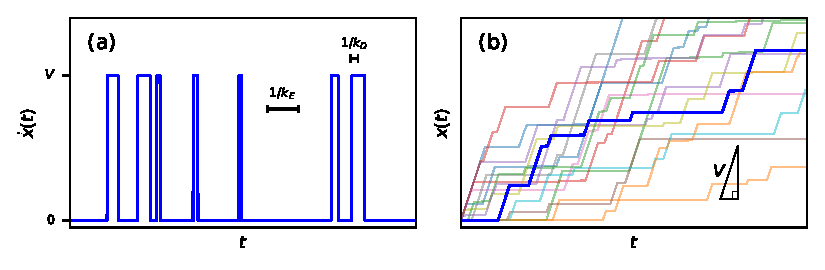
\includegraphics[width=\linewidth,keepaspectratio]{./figures/ch1/lisleConcept.pdf}
	\caption{Panel (a) indicates the generalization of Einstein's model to include the interval of sediment motion between entrainment and deposition, now represented with dichotomous noise eq. \ref{eq:lislerando}, while panel (b) shows the slanted stair-step trajectories of sediment particles moving downstream in cycles of motion at velocity $V$ (with mean duration $1/k_D$) and rest (which have mean duration $1/k_E$). }
	\label{fig:lislefig}
\end{figure}


For the intitial condition that particles have a probability $k_E/k$ to start in motion, the solution of equation \ref{eq:telegraph} is \citep{Lisle1998}
\be \ee
Incorporating the duration of sediment motion, the mean position of the sediment grain remains linear in time: $\langle x \rangle (t) = k_E V t/k$, representing movement at effective velocity $V_\text{eff} = k_E V/k$, which is the fraction of time spent in motion multiplied by the velocity during the motion phase. The variance, however, is different.
Computing $\sigma_x^2$ provides
\be \sigma_x^2(t) = ,\ee
which is a non-trivial result. At short times, for $t\ll 1/k$, equation \ref{eq:lislevar} shows diffusion $\sigma_x^2 \sim t^2$, which is a faster ``ballistic" rate of spreading than the Einstein model predicts \citep{Sokolov2014}. At long times ($t\gg 1/k$), the diffusion becomes normal again ($\sigma_x^2 = 2 D_\text{eff} t$), with an effective diffusion constant $ D_\text{eff} = k_E k_D V^2/k^3$.
In this model, both intermediate and global ranges are adequately represented, but local and geomorphic are not.

\subsection{The Newtonian approach}

Some authors have attempted to model local and intermediate ranges of individual particle trajectories by writing approximate Newtonian equations for the dynamics of individual particles and integrating them numerically. Early efforts impart particles with time-averaged fluid forces, typically linked to a logarithmic flow velocity profile \citep{VanRijn1984}, and some include simplified collision forces that modify particle velocities upon bed contact according to a set of simplified rules \citep{Wiberg1985,Sekine1992}.
Later on, researchers began to include granular interactions among particles to model collisions using the discrete element method \citep{Cundall1979, Haff1993}.
The early works utilizing this approach used a two dimensional domain with a highly simplified flow model \citep{Jiang1993}, while later works have included synthetic turbulence to drive particles \citep{McEwan2001,Schmeeckle2003,Maurin2015} or clever reduced-complexity representations of the flow \citep{Clark2015,Clark2017}.
The state of the art within this category of sediment transport models is to include two-way coupling between particles and the fluid flow. The latter is modelled either by large eddy simulation or direct numerical simulation of the Navier-Stokes equations, using particles as the boundary condition for the fluid \citep{Schmeeckle2014,Ji2013,Gonzalez2017,Vowincklel2014,Elghannay2017,Yousefi2020}.
A next step in this inquiry is to include non-spherical particles, and the foundation for this inquiry is now built \citep{Wachs2011, Azema2012, Wachs2019}.
These computational physics models produce impressive insight into the underlying granular and fluid physics mechanisms producing bed load transport \citep{Frey2011}, but analytically tractable models remain necessary for holistic understanding of sediment transport.

\subsection{Mechanistic-stochastic models for the sediment velocity distribution}
\label{sec:langevin}

The final set of models relevant to this thesis are the couple of analytical models that have been developed to describe particle velocities in the local and intermediate ranges when velocities fluctuate due to turbulence and particle-bed collisions. These models are indended to apply only between entrainment and deposition.
In contrast to the constant velocities introduced in section \ref{sec:lisle}, the velocities of bed load particles fluctuate through time and are best represented by statistical distributions. 
Among experimental studies on bedload velocities, two dominant conclusions have emerged. One subset of observations indicates that bedload velocities lie on exponential distributions \citep{Lajeunesse2010,Furbish2012,Fathel2015}, and another subset indicates Gaussian distributions \citep{Martin2012,Ancey2014,Heyman2016}.

\citet{Fan2014} set out to describe exponenential-distributed bedload particle velocities with a mechanistic model including a noisy driving term to represent fluid turbulence.
They wrote, for the streamwise particle velocity $u$, a Langevin equation
\be \dot{u}(t) = -\Delta \text{sgn}(u) + F + \sqrt{2D}\xi(t). \label{eq:fanlangevin}\ee
This equation drives the particle velocity by a fluid drag $F + \sqrt{2D} \xi(t)$, where $F$ is a constant, $D$ is a diffusivity that characterizes the magnitude of particle velocity fluctuations, and $\xi(t)$ is a Gaussian white noise with unit variance and vanishing mean \citep{Gardiner1983}. The fluid drag is resisted by a heuristic particle friction term $-\Delta \text{sgn}(u)$, introduced as a proxy for particle-bed collisions. The ``Fokker-Planck equation" governing the probability distribution $P(u,t)$ of the particle velocity can be derived from equation \ref{eq:fanlangevin} as \citep{Risken1984,VanKampen2007} 
\be \pt P(u,t) = \Delta\partial_u\Big[ \text{sgn}(u) P \Big] + D \partial_u^2 P,\ee
implying that the steady-state velocity distribution ($\pt P(x,t) = 0$) provided by equation \ref{eq:fanlangevin} is
\be P(u) = \frac{\Delta^2-F^2}{2\Delta D}\exp\Big(-\frac{-\Delta |u| + F u}{D}\Big).\ee
This is the (two-sided) exponential distribution observed in one subset of the aforementioned experiments.

In a similar approach, \citet{Ancey2014} formulated a Langevin equation to describe the Gaussian velocity distributions observed in the other subset of experiments. They wrote for the streamwise velocity 
\be t_r \dot{u}(t) = -(U-u) + \sqrt{2D}\xi(t),\ee
where $U$ is the mean velocity of particles, $D$ characterizes the magnitude of velocity fluctuations, and $\xi(t)$ is again a Gaussian white noise with vanishing mean and unit variance. The timescale $t_r$ is a relaxation time over which velocity fluctuations decay. This is the well-known Ornstein-Uhlenbeck process of stochastic physics \citep{Gardiner1983}, and its Fokker-Planck equation is
\be \pt P(u,t) = -\partial_u\Big[\frac{U-u}{t_r}P\Big] + \frac{D}{t_r^2} \partial_u^2 P.\ee
This time, the steady state solution becomes
\be P(u) = \sqrt{\frac{t_r}{2\pi D}} \exp\Big(-\frac{t_r(u-U)^2}{2 D}\Big), \ee
which is the Gaussian velocity distribution from the other subset of the experiments.

These models produce successful descriptions of disparate experimental results, although their components are not clearly interpretable in terms of physical expecatations. For example, granular interactions were included in the Fan et al model as a Coulomb friction term. While such approximations are common within Earth science models \citep{Kirkby1971}, they are not entirely satisfying given that bedload particles undergo intermittent collisions with the granular bed. Although these motions are sometimes described as ``sliding", bedload particles do not slide in the same sense as a block on a plane, as the granular term in the Fan et al Langevin model indicates.
In a similar way, the Ancey model does not have a particle-particle interaction term, and it includes what is apparently a Stokes drag term (linear in $u-U$), which is not applicable to bedload transport in water, since bedload particles are typically large compared to the viscous length scale \citep{Clift1978}.
We have to wonder if a more detailed treatment of particle-bed interactions might produce a more general model of bedload particle velocities for application at the local and intermediate scales.


\subsection{The definition of the flux}

Perhaps a surprising observation of bedload transport research is that no one definition of the sediment flux has even been agreed upon despite over a century of research \citep{Ballio2018}.
Today, there are two main competing (or complementary) approaches to define the bedload flux. 
The first definition is reminiscent of continuum mechanics and formulates the flux as a kind of current of sediment across a control surface $\matchal{S}$ \citep{Furbish2012,Heyman2016}: 
\be q = \int_\mathcal{S} c(\textbf{x},t)\textbf{u}\cdot d\textbf{\mathcal{S}}. \ee
This definition involves the concentration $c$ of particles in space and their velocites at the instant they cross the control surface, which is a somewhat elusive quantity since bedload particles are not a continuous field over the scales of interest \citep{Heyman2016}.
Lately, this concentration has been interpreted as an ensemble average \citep{Furbish2012,Ballio2014}.
The second definition formulates the downstream flux in terms of the number of particles moving within a control volume $\mathcal{V}$:
\be q = \frac{1}{L} \sum_{i\in\mathcal{V}} u_i. \label{eq:controlflux}\ee
Here, the flux is evaluated as a sum over all downstream velocities of particles within the volume (of which there are a fluctuating number), and the division by the downstream length of the control volume is incorporated to count only that proportion of particles near the downstream boundary of the volume.

An alternative statistical formulation of the sediment flux provides an approximate correspondence between these two definitions \citep{Ancey2006,Furbish2012}.
This alternative definition hinges on the probability $P[\textbf{u}_p | \textbf{x},t]$ that a particle contacts a control surface $S$ at position $\textbf{x}$ and time $t$ with velocity $\textbf{u}_p$. 
This conditional probability is considered to result from a very large collection of identical systems selected at random moments in their evolution: that is, the conditional probability is an ensemble quantity \citep{Kittel1958}.  

In terms of this ensemble probability, the flux is \citep{Ancey2006}: 
\be q_s = \int_{\text{all } \textbf{u}_p} \int_S P[\textbf{u}_p | \textbf{x},t] \textbf{u}_p \cdot d \textbf{S} d \textbf{u}_p . \label{eq:anceyflux} \ee
In steady conditions, when the probability is independent of time -- $\partial P / \partial t = 0$, the ensemble definition of the flux \ref{eq:anceyflux} can be approximated by the number of moving particles in the control volume. 

An approximate connection to a control volume flux can be derived by swapping the ensemble average for a spatial average, by integrating along a control volume.  
If the control volume is sufficiently long, $L \rightarrow \infty$, it can be seen as a stack of very many independent cross sectional surfaces. 
These comprise a stack of replicas of $\mathcal{S}$, and at an instant, if spatial correlations in bedload transport are weak, each surface constitutes one configuration of particles intersecting $S$ with some set of positions and velocities contributing to $P$. 
One can then define $P$ by counting occurrences along this stack of replica surfaces with an integral across the control volume.

With this concept of replica surfaces in mind, we can formalize the link with symbols. 
Consider $n$ particles distributed throughout a volume at some set of positions $\textbf{x}_i$ with some set of velocities $\textbf{u}_i$, where $i=0,1,\dots, n$,
The cloud of particles can be represented by its (discrete) density in a position-velocity phase space: 
\be \rho(\textbf{x},\textbf{u}_p) = \sum_{i=1}^n M(\textbf{x}-\textbf{x}_i)\delta^3(\textbf{u}_p - \textbf{u}_i). \ee  
Here $M(\textbf{z})$ is a marker function, which is $1$ if $\textbf{z}$ is inside the particle, and $0$ otherwise.
The marker's volume integral is $\int M(\textbf{x}) dV = \nu_p$, the particle volume. 

Using this density at sufficiently large $L$, the conditional probability $P[\textbf{u}_p | \textbf{x}]$ can be written approximately as an integral over the stack of replica surfaces:
\be P[\textbf{u}_p|\textbf{x}] \approx \frac{1}{L} \int_0^L dx \rho(\textbf{x},\textbf{u}_p). \ee
The integral runs along the downstream coordinate, and the equality becomes exact as $L \rightarrow \infty$.
With this swap of ensemble averaging for spatial averaging, the bedload flux becomes 
\be q_s \approx \int_{\text{all} \textbf{u}_p} \int_S \frac{1}{L} \int_0^L dx \sum_{i=1}^n M_a(\textbf{x}-\textbf{x}_i)\delta^3(\textbf{u}_p - \textbf{u}_i) \textbf{u}_p \cdot \textbf{k} dS d \textbf{u}_p = \frac{\nu_p}{L}\sum_{i=1}^n u_i , \ee
so there is some correspondence between the surface and volume definitions of the flux. Yet this is never exact, except in the unphysical case of sediment transport with no spatial correlations (vanishing particle size, discontinuous trajectories). Apparently, the control volume and control surface formulations of the sediment flux are not equivalent, so we see in the literature two parallel streams of research.

\subsection{The scaling arguments of Bagnold}

One of the most influential formulations of the bedload flux is due to Bagnold \citep{Bagnold1956,Bagnold1966}, who derived a formula for the mean sediment flux using an energy balance approach.
Bagnold understood sediment transport as a process which converts flow energy to heat via the effective friction \citep{Bagnold1954} of grains against the bed as they move downstream through a succession of collisions \citep{Bagnold1973}.
He assumed that the flow power $P_f$ available to move sediment scales as $P_f \propto \tau - \tau_c$, where $\tau$ is the average bed shear stress and $\tau_c$ is the threshold shear stress at which particles first begin to move. 
Considering that the average downstream flux of particles is $q$, and particles move with mean velocity proportional to the fluid velocity near the bed, Bagnold hypothesized that the power $P_g$ required to sustain particle motion scales as $P_g \propto q/\tau^{1/2}.$
 Balancing flow energy against frictional dissipation ($P_f = P_g$) then provides Bagnold's sediment transport formula
\be q = k(\tau-\tau_c)\tau^{1/2}, \label{eq:bagnold}\ee
which has shown good correspondence with laboratory data at large transport rates, given careful calibration of the constant factors $k$ and $\tau_c$.

The large shear stress limit $q \sim \tau^{3/2}$ of Bagnold's formula is shared in common with many other empirical formulas describing the mean downstream flux of bedload \citep[e.g.][]{MeyerPeter1948, Yalin1972, Wilcock2003, Parker1998}. The distinguishing feature of Bagnold's formula is its derivation from mechanical principles, although many of the details have since turned out to be incorrect. Bagnold's assumption that the power available to move sediment scaled with the excess shear stress leads to unphysical results over arbitrarily sloping beds \citep{Seminara2002}, and the flow power dissipated by sediment transport shows only a weak correlation the sediment flux \citep{Ancey2008}, while Bagnold assumed they were directly proportional. These issues have been hinted when calibrating Bagnold's formula to data, where the parameters $k$ and $\tau_c$ take on unphysical values at low transport rates \citep{Nino1996}.
More generally, Bagnold's formulation faces the notorious challenge of defining the critical shear stress $\tau_c$ for the initiation of sediment transport \citep{Paintal1971,Kirchener1990,Houssais2015,Clark2017,Allen2018}, which is a topic for another thesis. 
The difficulties with Bagnold's approach led to many revisions of his theory which kept Bagnold's sharp physical insights, but included new experimental conclusions on the energetics of sediment transport as they became available \citep{Engelund1976,Luque1976,Nino1998,Martin2000}.

\subsection{Einstein's probabilistic approach}

Among these revisions of Bagnold, one category shows a return to the probabilistic ideas of Einstein \citep{Parker2003,Ancey2006}.
Einstein formulated his original model of individual grains in transport \citep{Einstein1937} in terms of particle entrainment and deposition using the conceptual picture of grains moving downstream through a sequence of instantaneous steps.
Later, \citet{Einstein1942,Einstein1950} calculated the bulk sediment flux with these same probabilistic ideas, providing an alternative to the Bagnold scaling approach.
The conceptual picture that Einstein considered is depicted in figure \ref{fig:einsteinFluxConcept}.
 \begin{figure}[!htbp]
	\includegraphics[width=\linewidth,keepaspectratio]{./figures/ch1/yalinDrawing.pdf}
	\caption{Einstein’s conceptual picture (modified from \citet{Yalin1972}). Particles move in discrete jumps of length $\ell$ from
left to right through an array of adjacent control volumes. The bedload flux is the rate of bedload particles crossing
the surface $\mathcal{S}$ per unit width and time, collected from all upstream control volumes.}
	\label{fig:lislefig}
\end{figure}

He partitioned the channel into a sequence of identical control volumes $V$, and calculated the average rate at which particles cross a control surface by aggregating the contributions from each upstream control volume.
Each control volume has downstream length $\ell$ which is also the average particle step length.
Denoting by $P_n$ the probability that an individual grain undergoes at least $n$ jumps of length $\ell$ in a time interval $T$, meaning it travels at least a distance $n \ell$, and considering that there is a density $\rho$ of particles at rest on the bed, it follows that on average $\rho \ell P_n$ particles will displace a distance $n \ell$ or more from within each control volume during the time interval $T$. 
As a result, since grains crossing $\mathcal{S}$ in a time $T$ could have come from any upstream location, the number of grains crossing $\mathcal{S}$ in $T$ is a sum over all control volumes: $\sum_{n=1}^\infty \rho \ell P_n$.
Dividing by the time $T$ to get the average rate of grains crossing $\mathcal{S}$ provides the mean flux:
\be q = \frac{\rho \ell}{T} \sum_{n=1}^\infty P_n. \label{eq:einflux} \ee
The final quantity to evaluate is $P_n$, the probability a particle entrains \textit{at least} $n$ times in a time $T$.

Einstein originally constructed this probability by assuming that each particle had $n$ independent entrainment opportunities in the period $T$, each with probability $p$, so that $P_n = p^n$, giving $q \propto p/(1-p)$, but this approach has been revised by \citet{Yalin1972} and others \citep{Paintal1971,Cheng2004,Armanini2015,Armanini2017}. Some of these authors have argued that instead, one should calculate $P_n$ as an exceedance probability.
If the entrainment rate of an individual grain is $k_E$ (probability per unit time), then the probability that it entrains \textit{exactly} $n$ times in time $T$, denoted by $p_n$ (distinct from $P_n$!) is a Poisson distribution \citep{Cox1965}:
\be p_n = \frac{(k_E T)^n}{n!}e^{-k_E T}.\ee
This implies that the probability that it entrains \textit{at least} $n$ times is $P_n = \sum_{i=n}^\infty  \frac{(k_E T)^n}{n!}e^{-k_E T}, $
so Einstein's mean sediment flux (eq. \ref(eq:einflux}) becomes
\be q = \frac{\rho \ell}{T} \sum_{n=1}^\infty \sum_{l=n}^\infty = \frac{\rho \ell}{T}\sum_{n=1}^\infty n \frac{(k_E T)^n}{n!}e^{-k_E T} = \rho k_E \ell.\ee
Noticing that $\rho k_E$ is the entrainment rate of a single grain multiplied by the density of grains available for entrainment on the bed, we can summarize the Einstein theory as 
\be q = E \ell, \ee
where the quantity $E = \rho k_E$ is the ``areal entrainment rate", representing the number of grains entrained per unit bed area \citep{Wilcock1997,Furbish2012}.

Alongside this central result $q=E\ell$ for the mean flux, one of Einstein's most influential and enduring ideas was his formulation of the entrainment rate $k_E$ of the individual particle in terms of the force balance on the stationary particle.
The original approach considers that entrainment is driven by the fluctuating lift force imparted by the turbulent flow, and it is resisted by the submerged weight the grain.
The entrainment rate is calculated from the exceedance probability of the turbulent lift over the weight, providing an alternative to the critical shear stress concept which explicitly incorporates turbulent fluctuations in the fluid flow. This formulation of entrainment probability in terms of the exceedance of random driving quantities over (possibly
random) resisting quantities \citep{Grass1970} is a key part of Einstein's legacy. \citet{Paintal1971} made a significant extension
by including the random supporting geometry of bed particles into the force balance. More recently, \citet{Tregnaghi2012}
ammended the theory to include both force magnitude and duration \citep{Diplas2008, Valyrakis2012, Celik2014}.
Refined theories of the single-particle entrainment rate, all fundamentally similar to the original ideas of \citet{Einstein1950}, have been carefully reviewed by \citet{Dey2018} and are a topic under active development.

\subsection{Fusing Einstein and Bagnold: The erosion-deposition model}

Although Einstein worked to relate the single-particle entrainment rate $k_E$ to the flow, other parameters of Einstein's model ($\rho$, $\ell$) retain a heuristic character which is not clearly linked to the underlying fluid-granular physics.
The erosion-deposition model originally developed by \citet{Charru2004,Charru2006,Charru2006a} modifies the Einstein model and relates its parameters to properties of the flow using scaling relations obtained from experiments \citep{Charru2004, Charru2006, Lajeunesse2010,Seizilles2014,Lajeunesse2015}.
This can be characterized as a mixture of the Einstein and Bagnold strategies.

Derived by evaluating a mass balance within a control volume, the erosion-deposition model is
\be \pt \gamma +  \px V \gamma = E - D. \label{eq:charru}\ee
In this equation, $\gamma$ is the ``particle activity", which is the number of moving particles per unit area \citep{Furbish2012}, $V$ is the ensemble averaged movement velocity of sediment grains (which in unsteady conditions may depend on space and time), $E$ is the areal entrainment rate (the number of particles transitioning to motion per unit area and time), and $D$ is the areal deposition rate (the number of particles coming to rest on the bed per unit area and time).

Scaling arguments provide relations for $E$, $D$, and $V$ in terms of the fluid shear stress $\tau$, particle size $d$, particle settling velocity $V_s$, and critical shear stress $\tau_c$:
\be E = a \frac{\tau-\tau_c}{d^3 V_s}, \label{eq:charru1}\ee
\be D  = b\frac{\gamma V_s}{d}, \ee
\be V = c + d(\sqrt{\tau}-\sqrt{\tau_c}). \label{eq:charru2}\ee
The constant coefficients $a$, $b$, $c$, and $d$ are determined experimentally.

Equation \ref{eq:charru} indicates that the mean flux in steady transport conditions is the implicit solution to the equation $E = D.$
Using the scaling relations \ref{eq:charru1} and \ref{eq:charru2} provides the mean particle activity
\be \gamma \propto \frac{\tau-\tau_c}{d^2 V_s^2}.\ee
Expressing the mean flux as $q = \gamma V$, in the control volume interpretation, the relationship between flux and bed shear stress becomes
\be q = \frac{A}{d^2 V_s^2}\big(\tau-\tau_c\big)\big[c + d(\sqrt{\tau}-\sqrt{\tau_c})\big]. \ee
This recovers the Bagnold scaling $q \propto \tau^{3/2}$ at large bed shear stresses.

\subsection{The nonlocal formulation}

Einstein's model of the bulk bedload flux is inherently nonlocal in that it aggregates particle motions from all upstream locations \citep{Schumer2009}.
\citet{Parker2000} formalized this by writing the sediment flux in an explicitly nonlocal form:
\be q(x,t) = \int_0^\infty dx' F(x-x',t)E(x',t). \ee
In this equation, motions are instantaneous, and $F(x,t)$ is the probability that a just-entrained particle steps a distance $l$ before deposition.
This approach builds on Einstein because it can handle non-uniform conditions by space and time dependence of $E$ and $F$. 

\citet{Furbish2012} generalized the Parker model to include a finite duration of motion.
They wrote
\be q(x,t) = \int_0^\infty dx' \int_0^\infty dt' F(x',t') E(x-x',t-t'), \label{eq:furbo}\ee
where, $F(x,t)$ represents the probability density that particles move \textit{at least} a distance x in time $t$ (right after entrainment).
For a simple example of the Furbish et al formalism, consider that particles move with a constant velocity $V$ and have a deposition rate $k_D$. 
Then the probability density that a particle moves \textit{exactly} a distance $x$ in time $t$ is $f(x,t) = \delta(x-Vt)k_D\exp(-k_D t), $ so the probability that it moves 
\textit{at least} a distance $x$ in $t$ is
\be F(x,t) = \int_0^t \delta(x-Vt)k_D\exp(-k_D t) = \theta(Vt-x)k_D\exp(-k_D t).\ee
Considering uniform conditions with a density $\rho$ of particles available for motion on the bed surface, each having entrainment rate $k_E$, the bulk entrainment rate can be expressed as $E=\rho k_E$, and equation \ref{eq:furbo} provides a mean flux
\be q = \rho k_E \int_0^\infty dx' \int_0^\infty dt' \theta(Vt-x)k_D\exp(-k_D t) = \rho k_E V/k_D. \label{eq:furbflux}\ee
Since $1/k_D$ is the average time spent in motion, $V/k_D$ is the average step length $\ell$. Equation \ref{eq:furbflux} provides another perspective on Einstein's result $q= E\ell$.

\subsection{Landscape evolution}

Exner was probably the first to write the mathematical relationship between sediment transport and topographic change \citep{Exner1925}. He wrote
\be (1-\phi)\frac{\partial z}{\partial t}(\textbf{x},t) = -\nabla q (\textbf{x},t). \label{eq:exner}\ee
This equation links the temporal evolution of the land elevation $z$ at a location $\textbf{x}=(x,y)$ to spatial gradients in the sediment flux $q$. The parameter $\phi$ is the bed porosity.

Within the Exner equation, the elevation $z$ and sediment flux $q$ are represented as continuous fields. This representation can be interpreted as a spatial average over the detailed positions of individual grains, and it is expected to be valid whenever the scales of interest are large compared to the size of the averaging window, which is required to be be taken much larger than the size of the largest grains in the modelling domain \citep{Coleman2009}. 
Yet there are many Earth surface processes where the scale of interest is not much larger than the largest grains involved in the system. We can wonder, for example, how large boulders in mountain channels control the formation of steps \citep{Church2007,Zimmerman2008,Saletti2020}, or other bed structures having sizes comparable to channel widths, like ribs or stone cells \citep{Hassan2008,Venditti2017}. In these cases, individual grains are comparable to the scales of interest, and the continuum description provided by the Exner equation is not applicable.

\citet{Nakawaga1976} and \citet{Tsujimoto1978} developed an alternative statement of the Exner equation based upon Einstein's concepts of entrainment and deposition rates.
According to their formulation, spatial gradients in the sediment flux arise due to local discrepancies in entrainment and deposition:
\be \partial_x q(x,t) = E - D. \ee 
Owing to \ref{eq:exner}, this expression of the sediment flux immediately implies the ``entrainment form of the exner equation" \citep{Parker2000,Furbish2012,Fathel2015,Furbish2017} by which topographic evolution can be described in an Einstein-like framework: 
\be (1-\phi) px z(x,t) = D - E.\ee
In a nonlocal framework, as in equation \ref{eq:furbo}, sediment deposition can be interpreted as the result of entrainment at all upstream locations, giving
\be (1-\phi) px z(x,t) = \int_0^\infty \dx' int_0^\infty dt' E(x',t')F(x',t') - E(x,t). \ee
This ``entrainment form of the Exner equation" \citep{Furbish2017} phrases topographic change from a stochastic interpretation of sediment transport.

\subsection{Fluctuations and scale dependence}

Bedload flux signals exhibit characteristically large fluctuations \cite{Gomez1991,Bunte2005,Recking2012}, but all models reviewed to this point describe only mean sediment fluxes, and not the strength of bedload transport fluctuations, correlations, or other statistical characteristics of the flux.
A full statistical characterization of sediment transport is desirable because transport fluctuations are responsible for the initiation of bedforms \citep{Jerolmack2005,Bohorquez2016} and are beginning to show links to basic geomorphology considerations like the maintenance of stable channel widths \citep{Abramian2019,Abramian2020}.
This is not to mention that because sediment transport fluctuations are ubiquitous, models which describe only mean bedload fluxes signals are conceptually incomplete.

An additional reason to characterize fluctuations in bed load fluxes is because in reality, sediment flux measurements always involve a sampling interval.
This introduces questions of the convergence of transport rate measurements \citep{Dhont2018,Ancey2020}.
Fluctuations originate from processes which span a vast range of characteristic timescales.
These can occur over a matter of seconds, such as differences in the velocities of grains due to a series of collisions \citep{Benavides2021}, to many hundreds of hours, such as the migrations of dunes and bedload sheets \citep{Hammamori1962,Hoey1992,Guala2014} or the cycling between aggradation and degradation in pools \citep{Dhont2018}.
Such processes introduce temporal correlations into sediment transport signals which control the sampling interval over which measurements of the mean sediment flux converge \citep{Saletti2015,Singh2009,Singh2012}.
To date, very few modelling works have addressed the observation scale depedence of the bedload flux, whereby measurements of mean fluxes, or statistical moments, shift with observation time \citep{Ancey2020}.

\subsection{Birth death models for bedload flucuations}

The prevalence of large bedload fluctuations motivated \citet{Ancey2006,Ancey2008} to revisit Einstein's assumptions to develop a model of the bedload flux as a random variable.
They derived the probability distribution of this variable by counting the number of moving particles in a control volume. 
This number changes through time as a result of entrainment and deposition.
To obtain realistically-wide fluctuations in particle activity, they introduced a positive feedback called ``collective entrainment", whereby the entrainment rate of grains increases in proportion to the number of moving grains in the volume \citep{Ancey2008,Heyman2013}.

Their governing equations are completely analogous to a stochastic population model \citep{Cox1965, Pielou1977} where entrainment is ``birth" and deposition is ``death".
They formulated the probability mass function $P(n,t)$ of the number of moving grains in the control volume at time $t$ as
\be \pt P(n,t) = \big[\lambda + (n-1)\mu\big] P(n-1,t) - [n+1]\sigma P(n+1,t) - \big[\lambda + n (\sigma + \mu)\big],\ee
whose terms describe entrainment at rate $\lambda$, collective entrainment at rate $\mu$, and deposition at rate $\sigma$. 
The final term encodes the possibility that $n$ does not change at a given instant.
These coupled equations (one for each $n=0,1,\dots$) can be solved by generating functions \citep{Cox1965,Ancey2008}, providing the steady-state distribution
\be P(n) = \frac{\Gamma(r+n)}{\Gamma(r) n!}p^r(1-p)^n, \label{eq:negbin}\ee
where $r = \lambda/\mu$ and $p = 1-\mu/\sigma$.
This is a negative binomial distribution, which is a wide-tailed generalization of the Poisson distribution. 

From eq. \ref{eq:negbin}, the mean number of moving particles is $\langle n \rangle = \lambda/(\sigma-\mu)$, and the variance is
\be \sigma_n^2 = \frac{\lambda \sigma}{(\sigma-\mu)^2}. \ee
Owing to the collective entrainment process, particle activity fluctuations can be arbitrarily wide: $\sigma_n/\bra n \ket = \sqrt{\sigma/\lambda}$, whereas in the absence of collective entrainment ($\mu=0$), the strength of fluctuations is always pinned to 1, as the distribution \ref{eq:negbin} limits to a Poisson distribution \citep{Ancey2006}.

The probability distribution of the bedload flux can be computed by the control volume form, eq. \ref{eq:controlflux} given, in addition, the probability distribution of particle velocites, which can be determined experimentally \citep{Lajeunesse2012,Fathel2015,Heyman2016} or calculated using the Langevin models described in section \ref{sec:langevin}.
Assuming that the particle activity in the control volume and the velocities of moving particles are completely independent, which may be a good assumption for a large enough control volume, the probability distribution $Q(q)$ of the flux is \citep{Ancey2008,Ancey2014,Ancey2020}
\be Q(q) = L \sum_{k=1}^\infty P(k)G(U) ,\ee
where $P(n)$ comes from eq. \ref{eq:negbin} and $G(U)$ is the probability that the sum of $k$ particle velocities at some instant is equal to $U$.

\subsection{Renewal theories for scale dependence}

The final approach to summarize is that of \citet{Ancey2020}, which calculates the sediment flux probability distribution from an ``arrival time distribution" representing the distribution of times between subsequent arrivals of particles to a control surface. This distribution changes depending on the observation time $T$ used to calculate the averaged flux. This is the phenomenon of scale dependence.

 \begin{figure}[!htbp]
	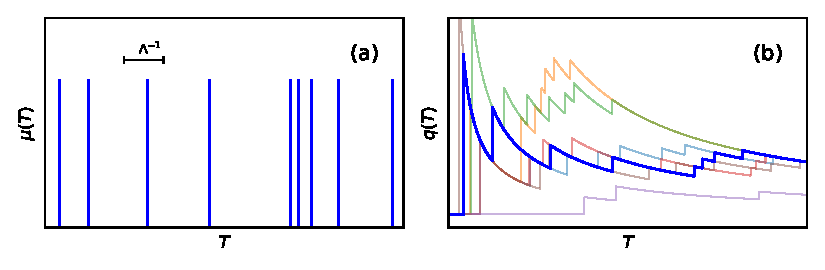
\includegraphics[width=\linewidth,keepaspectratio]{./figures/ch1/anceyRenewal.pdf}
	\caption{The scale-dependent sediment flux is described as a renewal process. Panel (a) indicates the arrivals of particles at rate $\Lambda$, while panel (b) shows an ensemble of realizations of the sediment flux versus the observation time $T$. Note that different realizations of the flux converge toward the same value at large observation times, whereas at small observation times, uncertainty in the flux is large. This is observation-scale dependence. The nature of this convergence depends on the particle dynamics in an as yet unspecified way. }
	\label{fig:ancey}
\end{figure}

\citet{Ancey2020} considered two different arrival time distributions to calculate the probability distribution of the time-averaged sediment flux. Only the first of these is reviewed here. This is an exponential distribution: $P(t) = \Lambda \exp(-\Lambda t),$ so the mean time between particle arrivals is $1/\Lambda$.
In this case, the flux averaged over a period $T$ can be represented with a Poisson pulse noise, similar to the particle position in the Einstein model of section \ref{sec:einstein}:
\be q(T) = \frac{1}{T}\int_0^T dt' \mu(t'). \label{eq:flucflux}\ee
Here, the noise is 
\be \mu(t) = \sum_{i=1}^{N(t)}\delta(t-t_i), \label{eq:poissfluxnoise}\ee
as indicated in figure \ref{fig:ancey} panel (a). In this equation, $N(t)$ is Poisson distributed with rate $\Lambda t$. 
The flux in eq. \ref{eq:flucflux} is a random variable as indicated in \ref{fig:ancey} panel (b). Its probability distribution, which is contingent on the observation time $T$, can be derived by evaluating $P(q|T) = \bra \delta(q-\int_0^T \mu(t') dt'/T) \ket$. This equation entails an average over all possible realizations of the noise in eq. \ref{eq:poissfluxnoise}, producing \citep{VanKampen2007}
\be  \ee


\section{Open problems and thesis outline}


\endinput

